\begin{figure}
	\begin{subfigure}{\linewidth}
		\centering
		\begin{adjustbox}{height=.7\textwidth}
			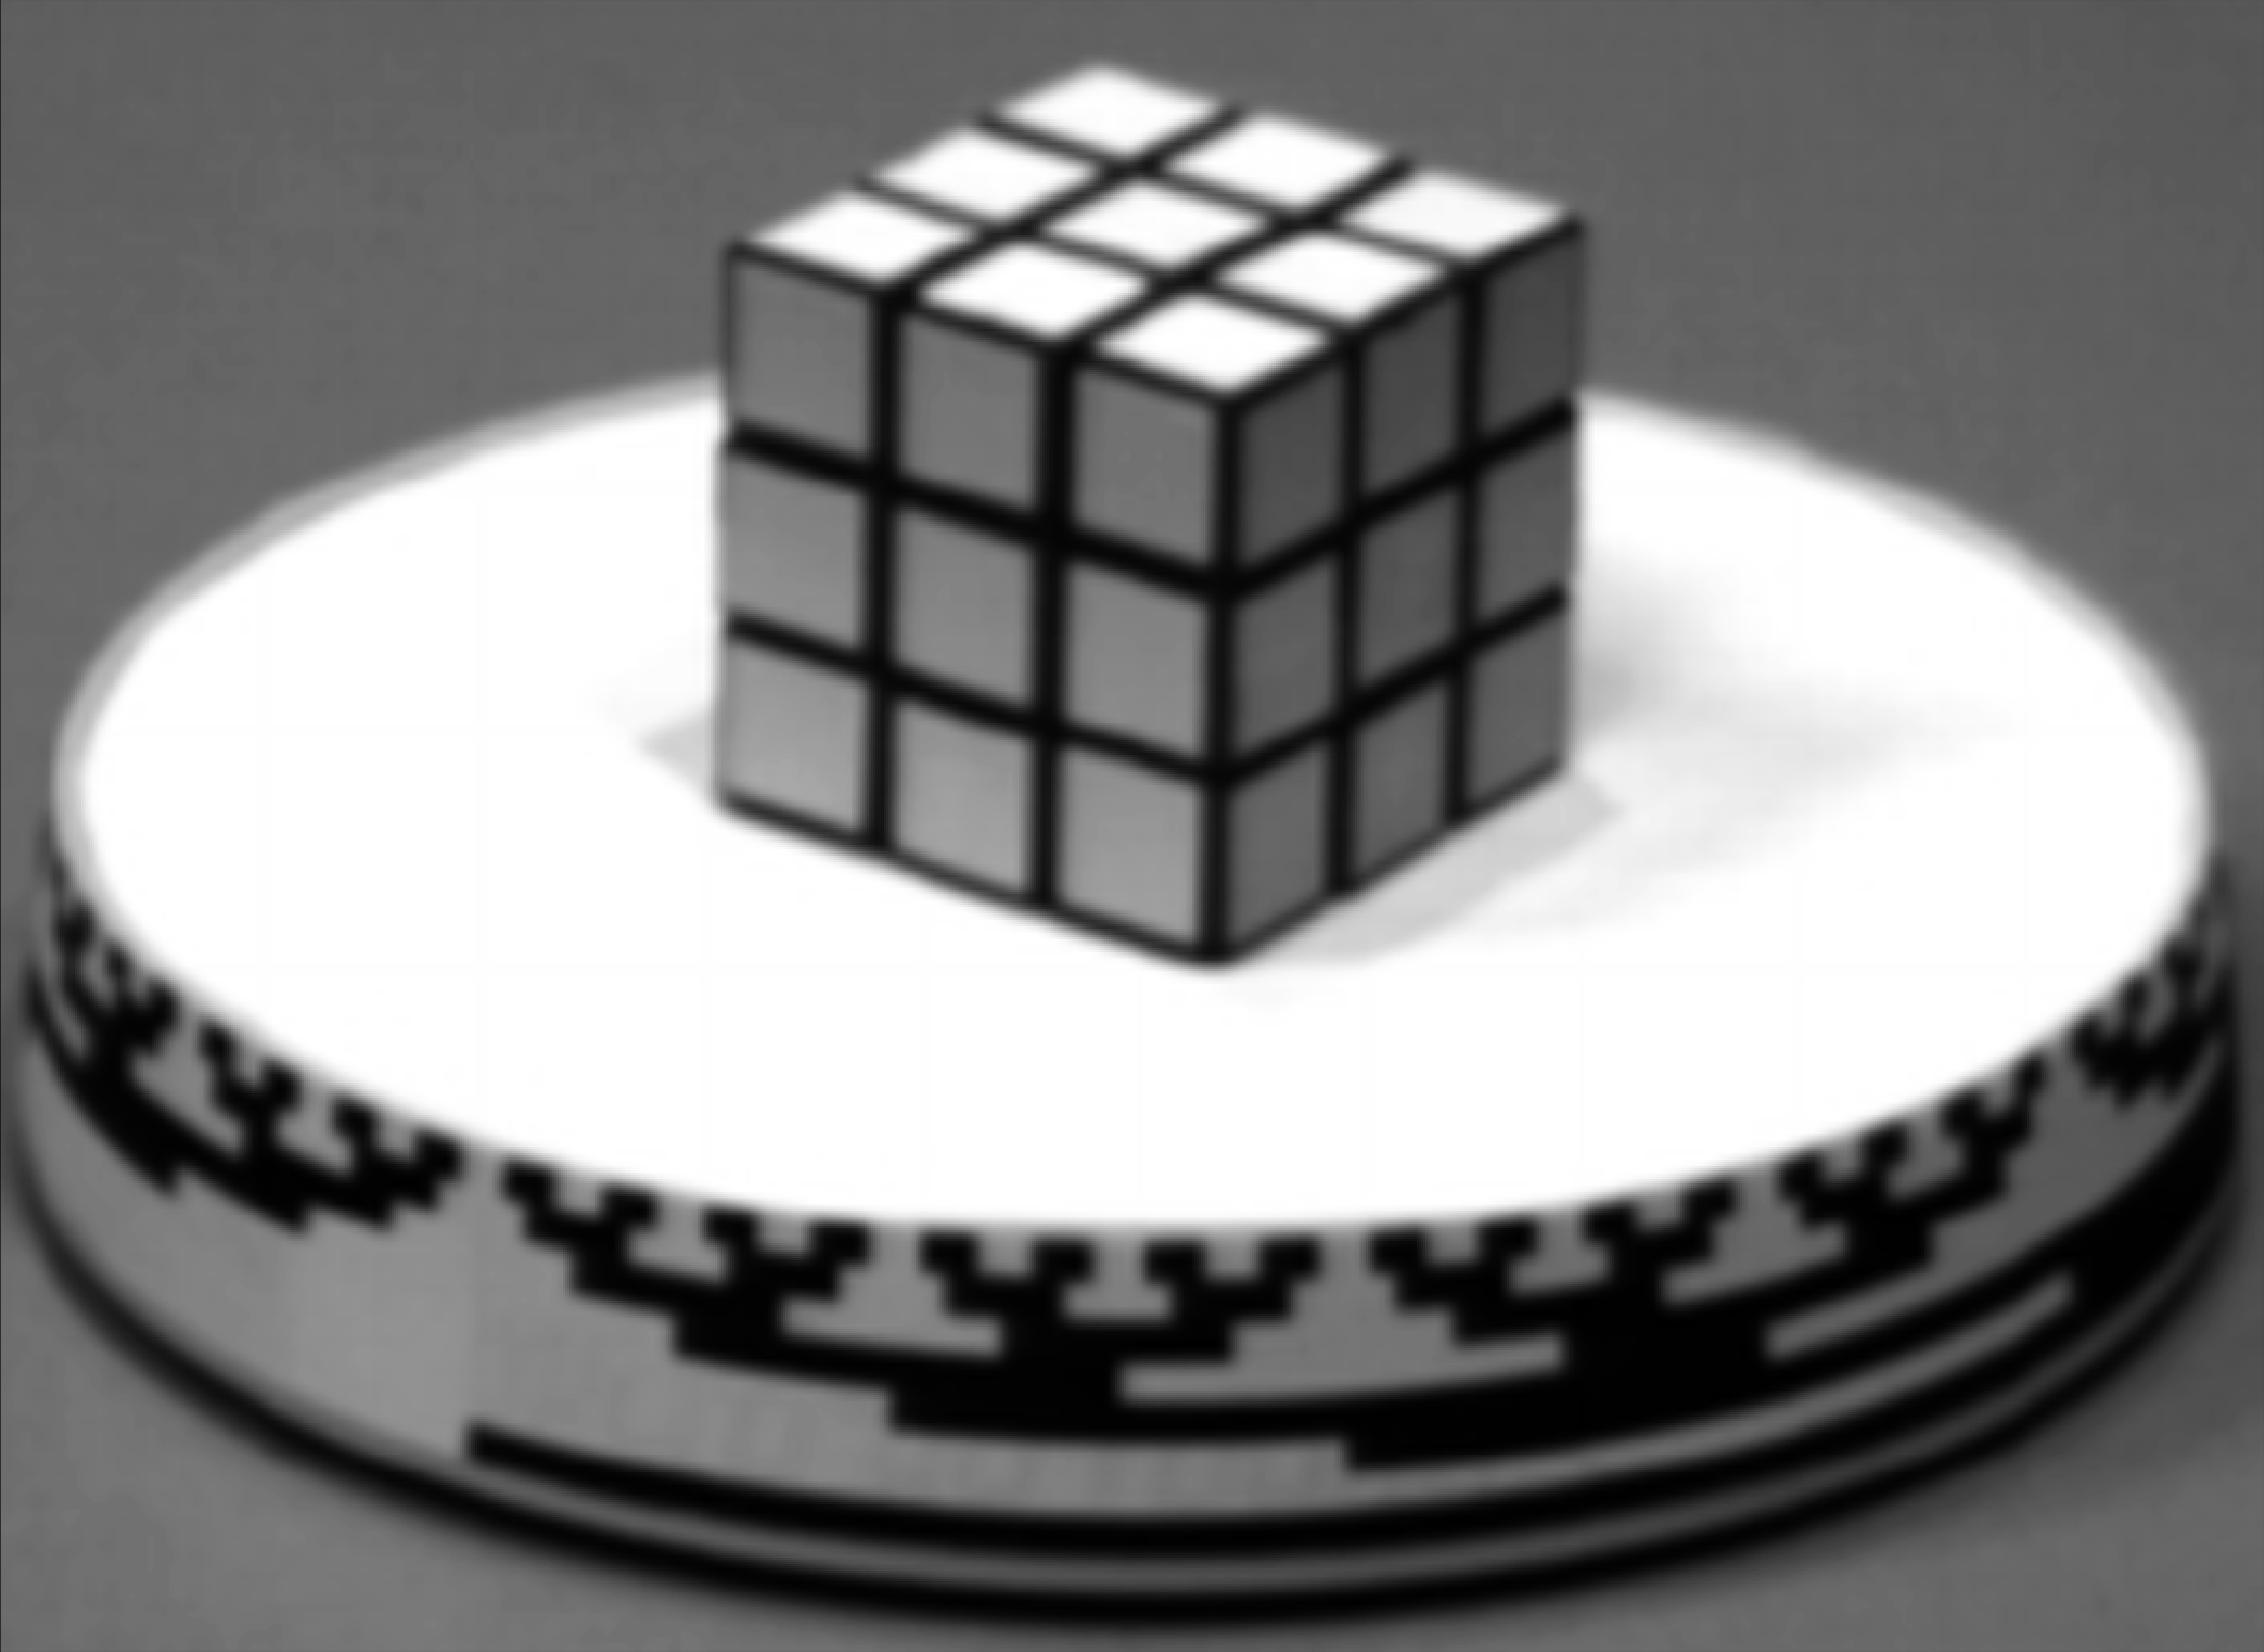
\includegraphics[]
			{figures/registration/optical_flow/reference_image.png}
		\end{adjustbox}
		\caption{Reference image} \label{fig:refoptical}
	\end{subfigure}
	\vskip\baselineskip
	\begin{subfigure}{\linewidth}
		\centering
		\begin{adjustbox}{height=.7\textwidth}
			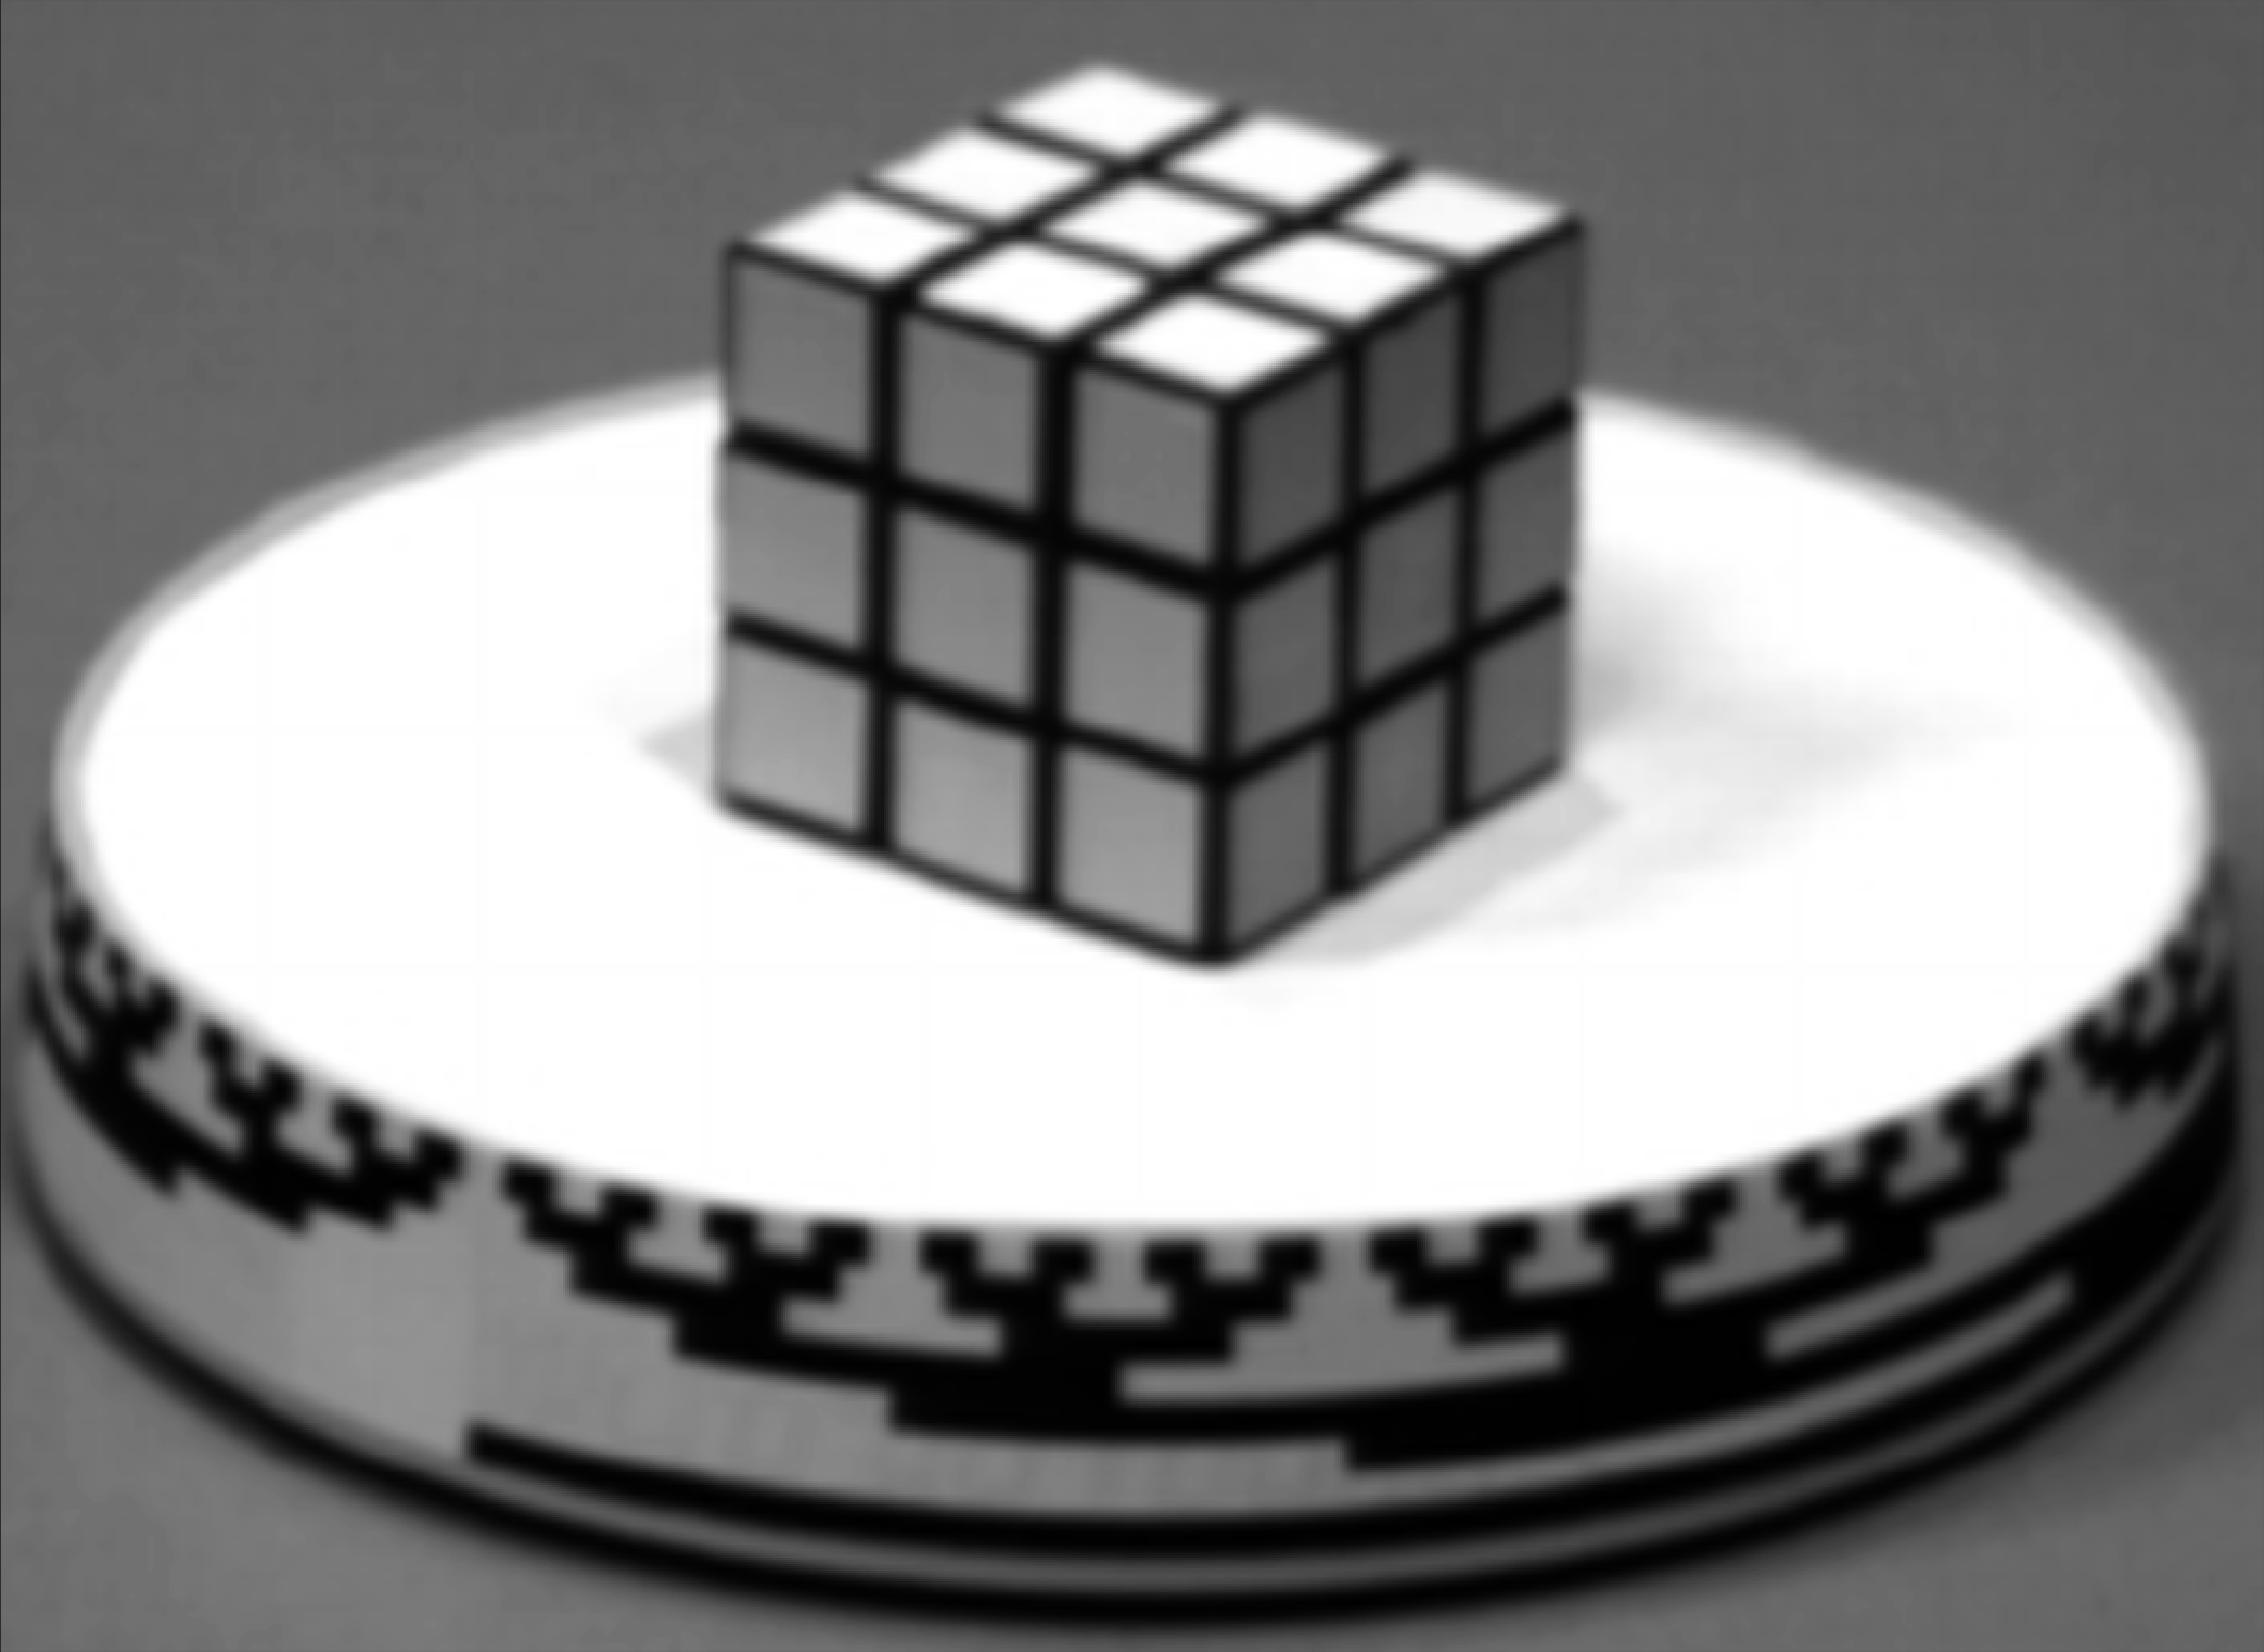
\includegraphics[]
			{figures/registration/optical_flow/moving_image.png}
		\end{adjustbox}
		\caption{Moving/displaced image} \label{fig:movoptical}
	\end{subfigure}
	\vskip\baselineskip
	\begin{subfigure}{\linewidth}
		\centering
		\begin{adjustbox}{height=.7\textwidth}
			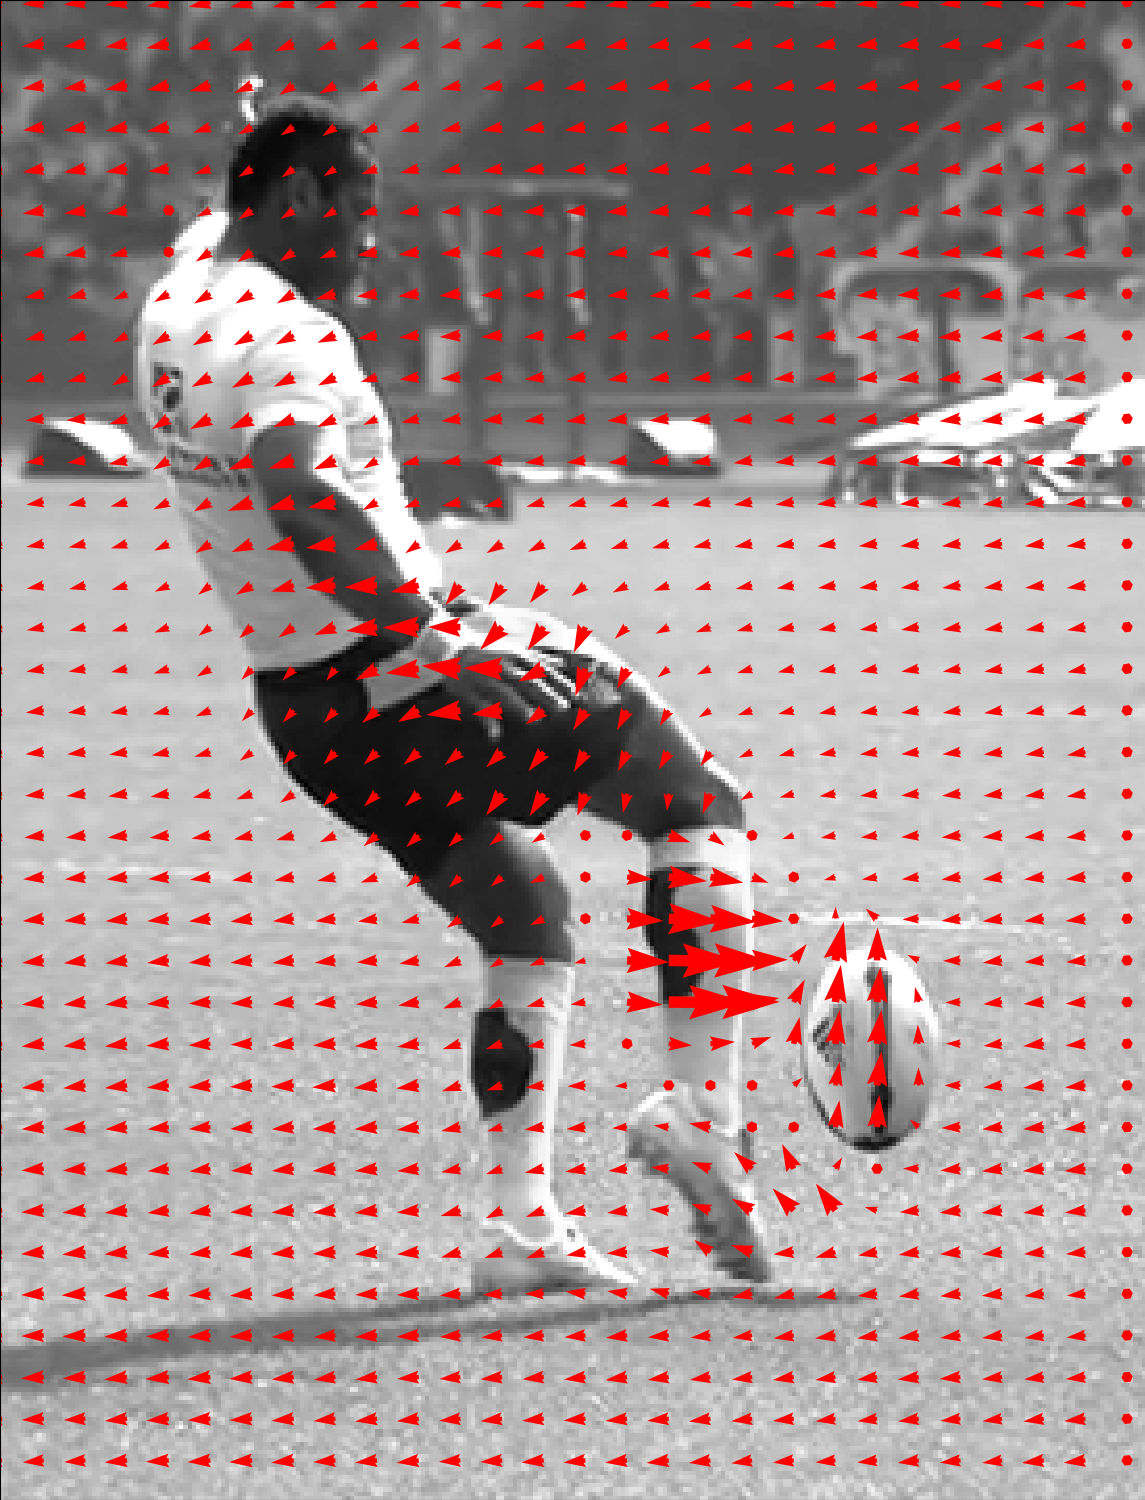
\includegraphics[]
			{figures/registration/optical_flow/flow.png}
		\end{adjustbox}
		\caption{Velocity field} \label{fig:fieldoptical}
	\end{subfigure}
	\caption{Optical flow}
	\label{fig:opticalflow}
\end{figure}
